\chapter{Autoencoder}

Un \textbf{Autoencoder} è una rete neurale progettata per apprendere una rappresentazione compressa dell’input attraverso un processo di codifica e successiva decodifica, con l’obiettivo di ricostruire fedelmente l’input stesso in output: $h_\theta (x) \approx x$. Sebbene questa formulazione possa apparire banale, il valore dell'autoencoder risiede nella sua capacità di apprendere rappresentazioni utili dei dati grazie a specifici vincoli architetturali. In particolare, l’apprendimento di una funzione identità approssimata diventa un compito non banale se si impongono vincoli strutturali quali:

\begin{enumerate}
\item \textbf{Compressione del livello nascosto}: La dimensionalità dello strato nascosto è inferiore rispetto a quella dell’input, costringendo la rete a catturare le caratteristiche più rilevanti dell’informazione.
\item \textbf{Sparsità}: Si introduce un vincolo per cui, durante la fase di training, solo un numero limitato di neuroni dello strato nascosto risulta attivo per ogni input. Ciò viene realizzato aggiungendo un termine di penalizzazione alla funzione di costo.
\end{enumerate}

\begin{figure}[h!]
\centering
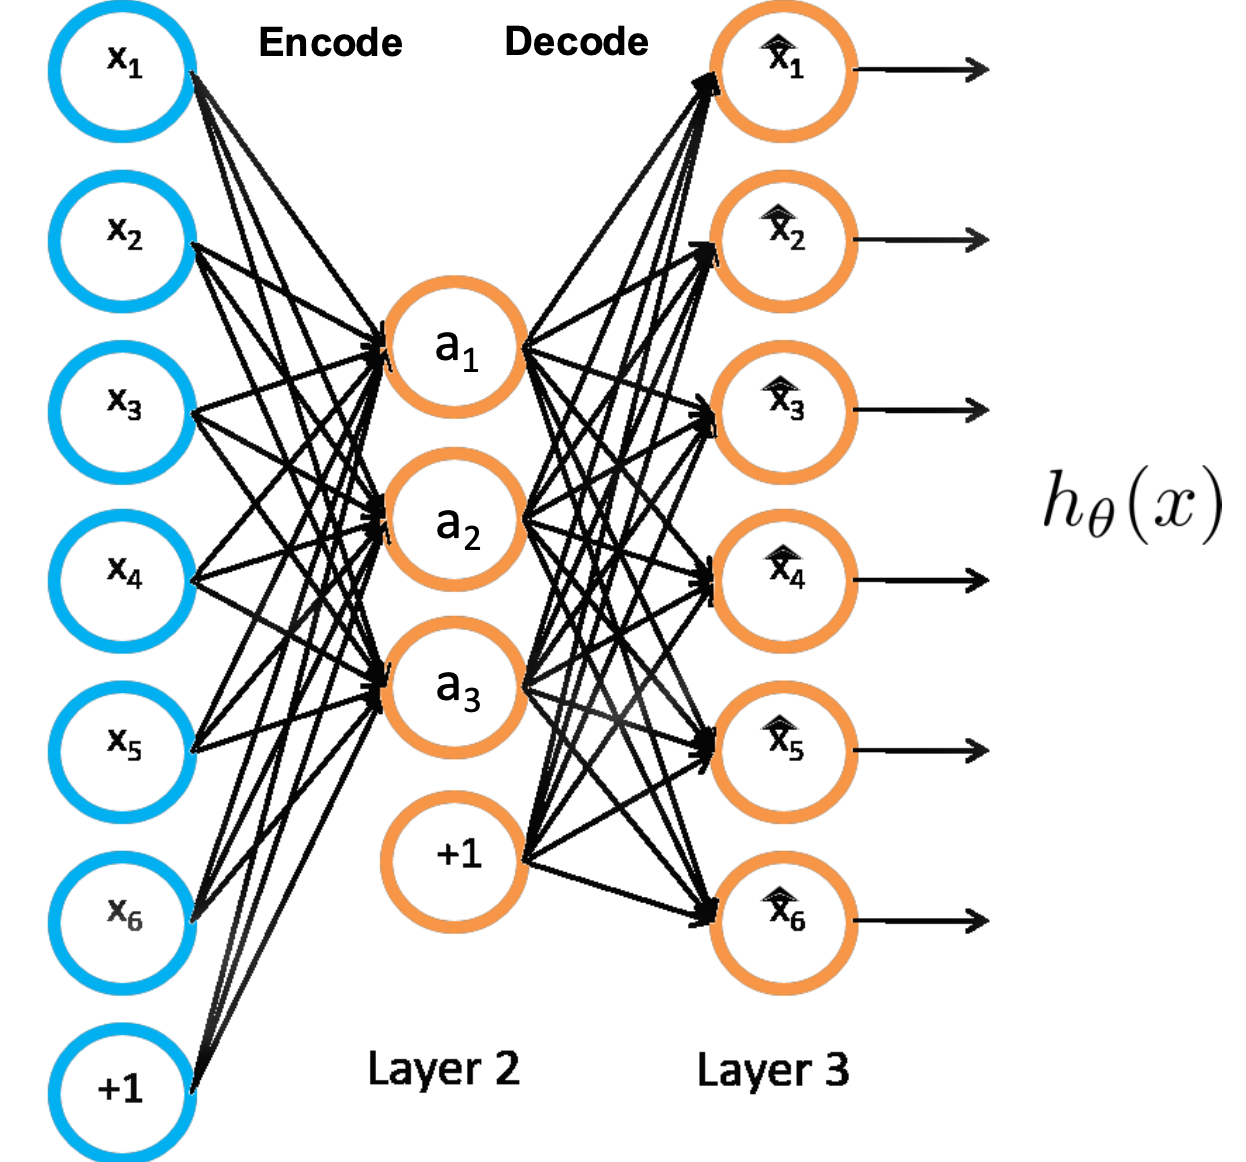
\includegraphics[width=0.5\textwidth]{figure/AAutoencoder.png}
\caption{Struttura tipica di un Autoencoder}
\label{fig:AutoEnc}
\end{figure}

\section{U-Net}

La \textbf{U-Net} è un’architettura di deep learning sviluppata specificamente per compiti di segmentazione semantica di immagini, con applicazioni rilevanti in ambito medico, come l’identificazione di lesioni o tumori. L’obiettivo è classificare ogni singolo pixel dell’immagine in una determinata categoria, restituendo una mappa binaria o multiclasse. Un esempio è illustrato in Figura~\ref{fig:cell}.

\begin{figure}[!ht]
\centering
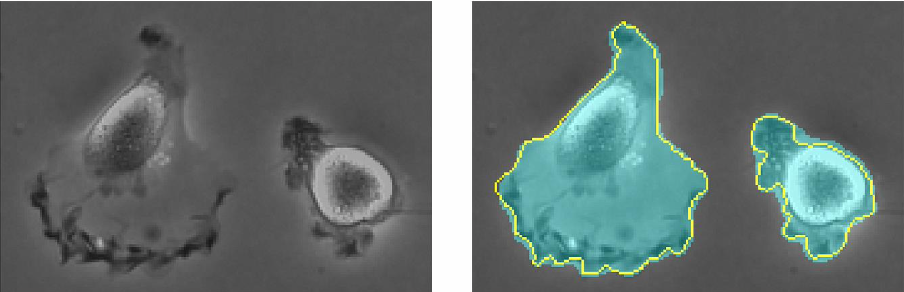
\includegraphics[width=0.75\textwidth]{figure/Cells.png}
\caption{Esempio di segmentazione semantica: a sinistra l'immagine originale, a destra la mappa segmentata. I pixel evidenziati rappresentano la classe target.}
\label{fig:cell}
\end{figure}

L’architettura della U-Net è suddivisa in tre componenti principali: \emph{Encoder}, \emph{Decoder} e \emph{Skip Connections}.

\begin{itemize}
\item \textbf{Encoder}: Composto da blocchi convoluzionali e operazioni di downsampling (es. max pooling), estrae progressivamente feature sempre più astratte.
\item \textbf{Decoder}: Costituito da operazioni di upsampling (es. up-convolutions) e convoluzioni, ricostruisce l’immagine nella sua risoluzione originale.
\item \textbf{Skip Connections}: Collegano simmetricamente gli strati dell’encoder con quelli del decoder, trasmettendo direttamente informazioni spaziali dettagliate, utili alla ricostruzione dell’output.
\end{itemize}

\begin{figure}[!ht]
\centering
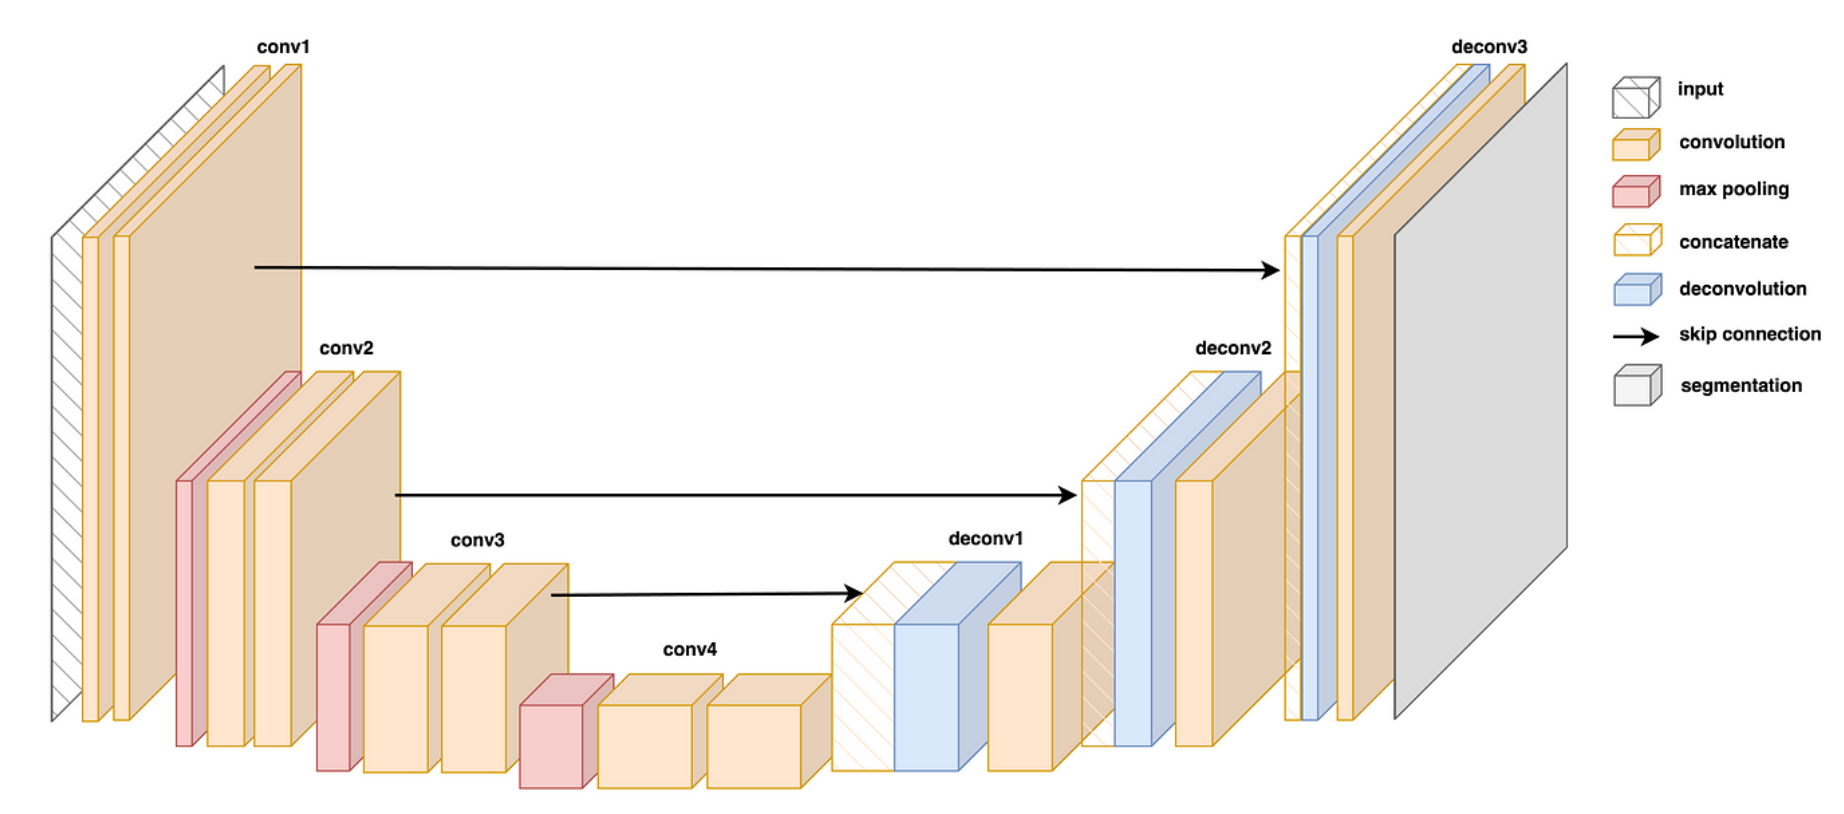
\includegraphics[width=0.85\textwidth]{figure/UNet.png}
\caption{Architettura di una U-Net}
\label{fig:unet}
\end{figure}

Durante la fase di downsampling, le informazioni spaziali precise tendono a degradarsi. Tuttavia, grazie alle skip connections, le caratteristiche di basso livello, conservate nei primi layer convoluzionali, vengono riutilizzate nel decoder per preservare la localizzazione spaziale dei dettagli. Questo migliora sensibilmente la qualità dell'output segmentato.

\section{Limitazioni degli Autoencoder}

Gli autoencoder sono efficaci per compiti di compressione, riduzione del rumore e apprendimento non supervisionato. Tuttavia, presentano alcune limitazioni nel contesto generativo. In particolare, lo spazio latente appreso non è strutturato in modo tale da garantire la generazione di nuovi esempi coerenti.

\begin{figure}[!ht]
\centering
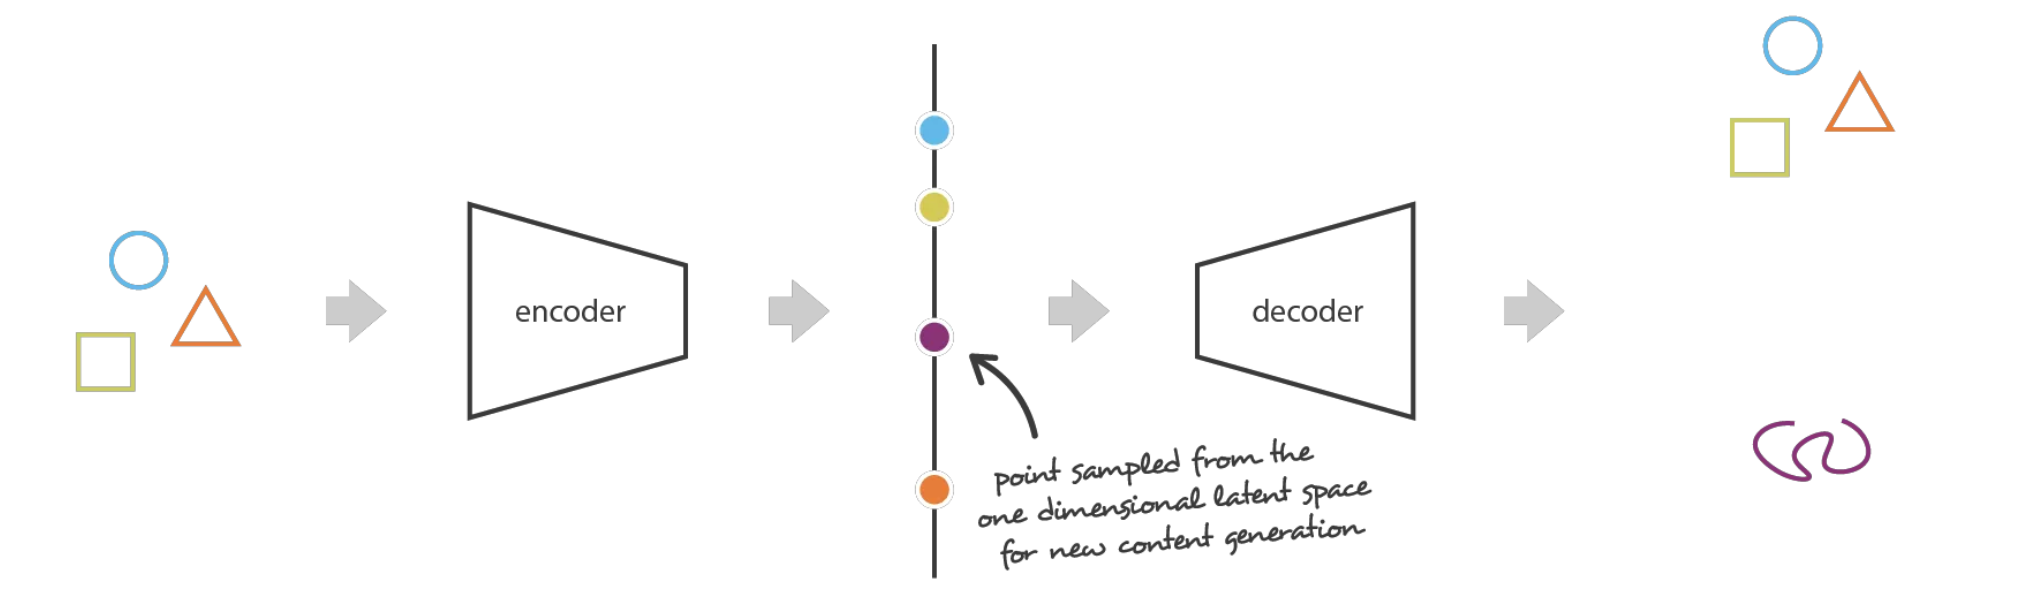
\includegraphics[width=\textwidth]{figure/EncLimit.png}
\caption{Distribuzione irregolare nello spazio latente: regioni inutilizzate o contenenti rumore}
\label{fig:enclimit}
\end{figure}

L’encoder può infatti mappare gli input in regioni isolate del latent space, lasciando vaste aree vuote. Ciò implica che, campionando casualmente un punto in questo spazio, è probabile ottenere un output privo di significato. Inoltre, non vi è garanzia che interpolazioni lineari tra due punti "validi" generino anch’esse esempi coerenti.

\section{Variational Autoencoder (VAE)}

Il \textbf{Variational Autoencoder} (VAE) è un’estensione probabilistica dell’autoencoder classico. Esso introduce una regolarizzazione nello spazio latente per consentire una generazione di dati coerente e continua. A differenza degli autoencoder tradizionali, i VAE non codificano l’input come un singolo punto nello spazio latente, ma come una distribuzione di probabilità. Il processo di training coinvolge i seguenti passaggi:

\begin{enumerate}
\item L’encoder mappa l’input in una distribuzione probabilistica (tipicamente gaussiana);
\item Viene campionato un punto da questa distribuzione;
\item Il decoder ricostruisce l’input a partire da tale punto;
\item L’errore di ricostruzione viene propagato all’indietro.
\end{enumerate}

La funzione di perdita del VAE combina due componenti, uno è il termine di ricostruzione che penalizza la differenza tra input e output, l'altro è un termine di regolarizzazione, la divergenza di Kullback-Leibler tra la distribuzione appresa e una distribuzione normale standard.

\begin{equation}\begin{split}
\mathcal{L} = \| x - \hat{x}\|^2 + \operatorname{KL}[\mathcal{N}(\mu_x,\sigma_x), \mathcal{N}(0,\operatorname{I})] =\\= \|x-\operatorname{d}(z)\|^2 + \operatorname{KL}[\mathcal{N}(\mu_x,\sigma_x), \mathcal{N}(0, \operatorname{I})]
\end{split}
\end{equation}

\subsection{Proprietà desiderate dello spazio latente}

Un buon spazio latente per la generazione di dati deve soddisfare le seguenti proprietà:

\begin{itemize}
\item \textbf{Continuità}: Piccole variazioni nel latent space devono produrre output simili;
\item \textbf{Completezza}: Qualsiasi punto dello spazio latente dovrebbe decodificarsi in un output plausibile.
\end{itemize}

Tali proprietà non sono garantite automaticamente. Le difficoltà principali includono:

\begin{itemize}
\item Encoding inadeguato: distribuzioni malformate o disgiunte non assicurano continuità o completezza.
\item Mancata regolarizzazione: il VAE può comportarsi come un autoencoder classico.
\item Distribuzioni con varianza trascurabile: rendono l’encoding troppo deterministico.
\item È necessaria una regolarizzazione sia della media che della covarianza.
\end{itemize}

\begin{figure}[!ht]
\centering
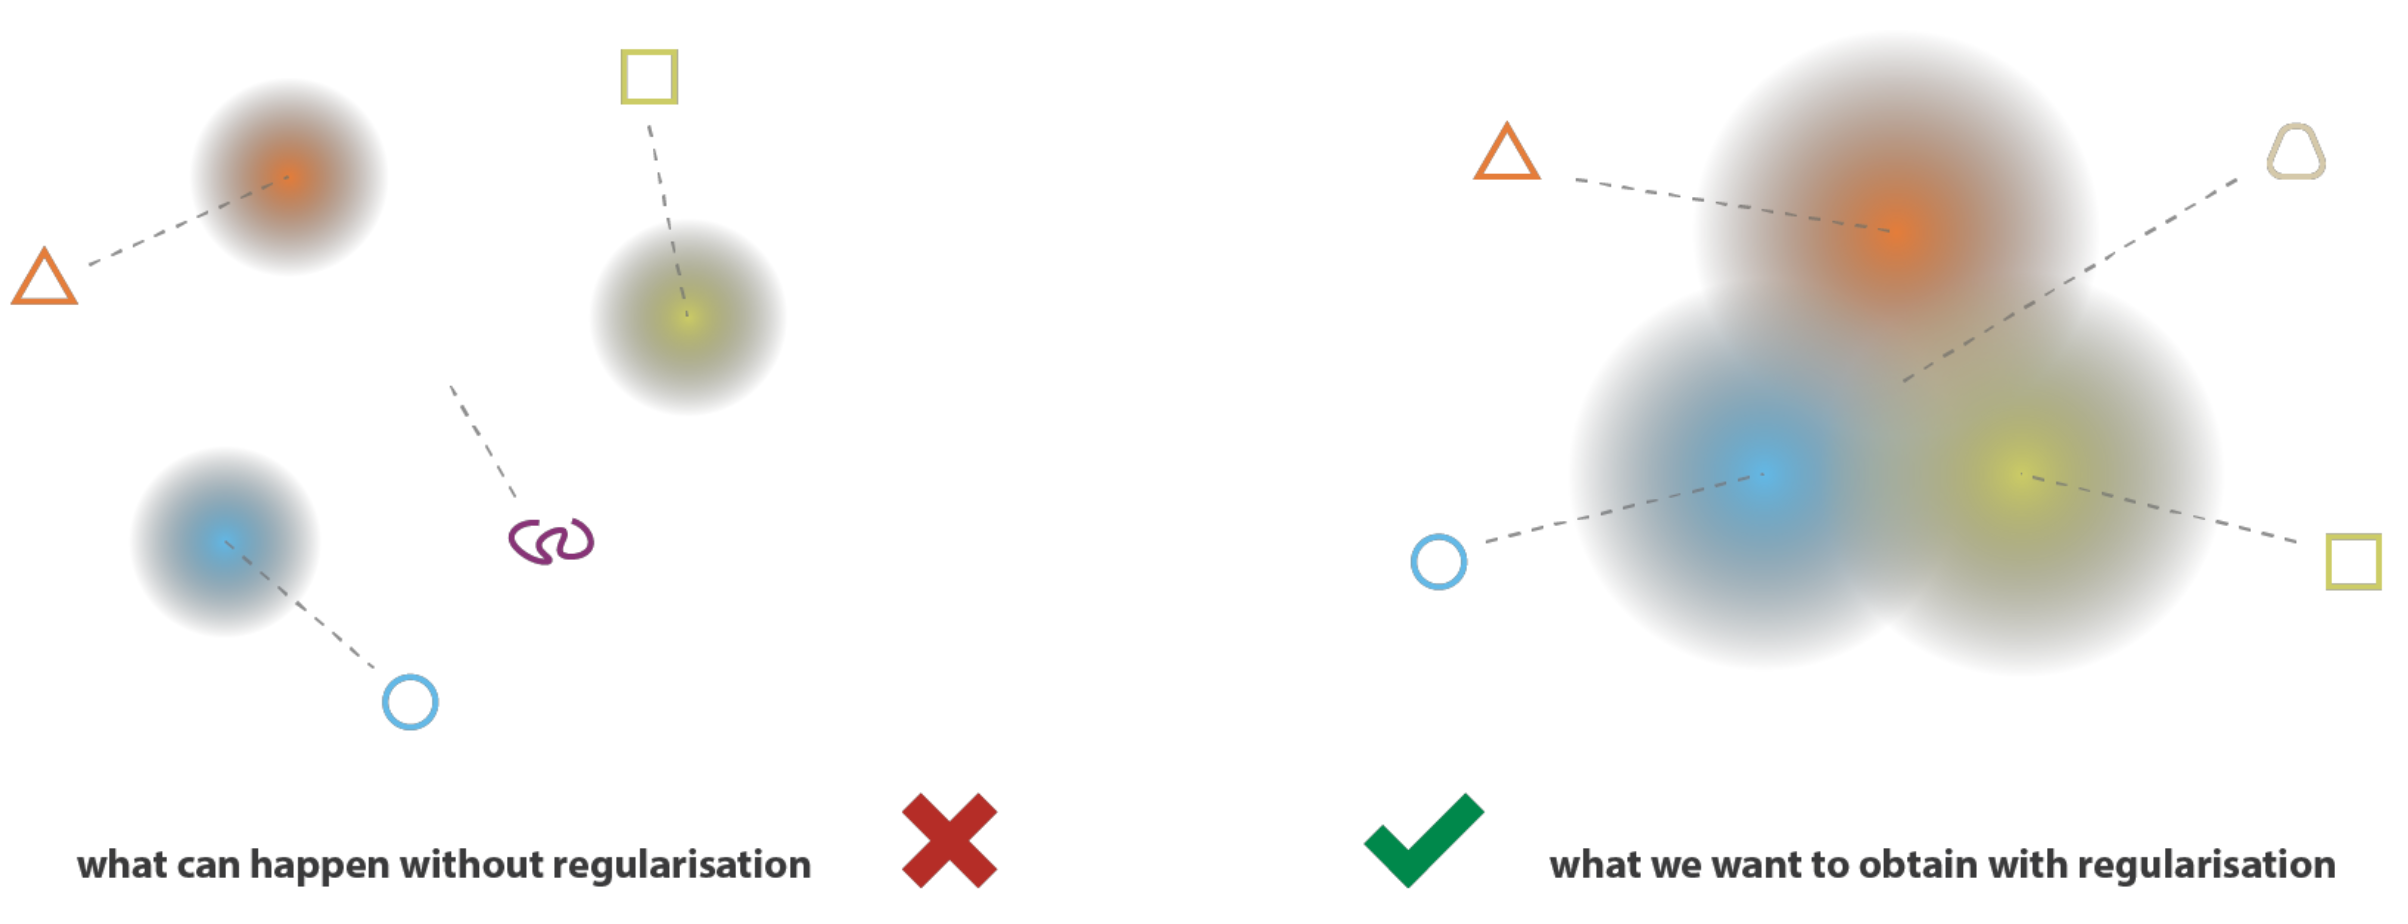
\includegraphics[width=\textwidth]{figure/RegEnc.png}
\caption{Effetti della regolarizzazione nello spazio latente}
\label{fig:regEnc}
\end{figure}

\section{Visione probabilistica dei VAE}

Consideriamo $x$ un input e $z$ una variabile latente. L’obiettivo del VAE è apprendere un modello generativo che consenta di generare nuovi campioni $x$ campionando da una distribuzione a priori su $z$, tipicamente $\mathcal{N}(0, I)$. La generazione avviene tramite:

\begin{itemize}
\item Campionamento di $z \sim p(z)$;
\item Campionamento di $x \sim p(x|z)$.
\end{itemize}

La distribuzione $p(x|z)$ è il \textit{decoder probabilistico}, mentre $p(z|x)$ è l'\textit{encoder probabilistico}. Quest’ultima risulta spesso intrattabile poiché implica il calcolo dell’integrale di marginalizzazione:

\begin{equation}
p(z|x) = \frac{p(x|z),p(z)}{p(x)} \quad,\quad p(x) = \int p(x|z),p(z),dz
\end{equation}

\subsection{Inferenza variazionale}

Per affrontare questa difficoltà, si ricorre all’\textbf{inferenza variazionale}, approssimando $p(z|x)$ con una distribuzione $q_x(z)$ scelta all’interno di una famiglia parametrica (es. gaussiana). La media e la varianza di $q_x(z)$ vengono apprese tramite funzioni $g(x)$ e $h(x)$:

\begin{equation}
\max_{(f,g,h)} \left( \mathbb{E}_{z\sim q_x}\left[-\frac{|x - f(z)|^2}{2c}\right] - \operatorname{KL}(q_x(z),|,p(z)) \right)
\end{equation}

L’obiettivo è minimizzare la distanza tra $q_x(z)$ e $p(z)$, garantendo al contempo una buona ricostruzione dell’input.

\subsection{Reparametrization Trick}

Il campionamento da $q_x(z) = \mathcal{N}(\mu_x, \sigma_x)$ non è differenziabile, impedendo l’uso diretto della backpropagation. Il \textbf{reparametrization trick} risolve questo problema: si campiona un vettore $\zeta \sim \mathcal{N}(0,I)$ e si imposta $z = \mu_x + \sigma_x \cdot \zeta$. In questo modo, il campionamento diventa un'operazione differenziabile.

\begin{figure}[!ht]
\centering
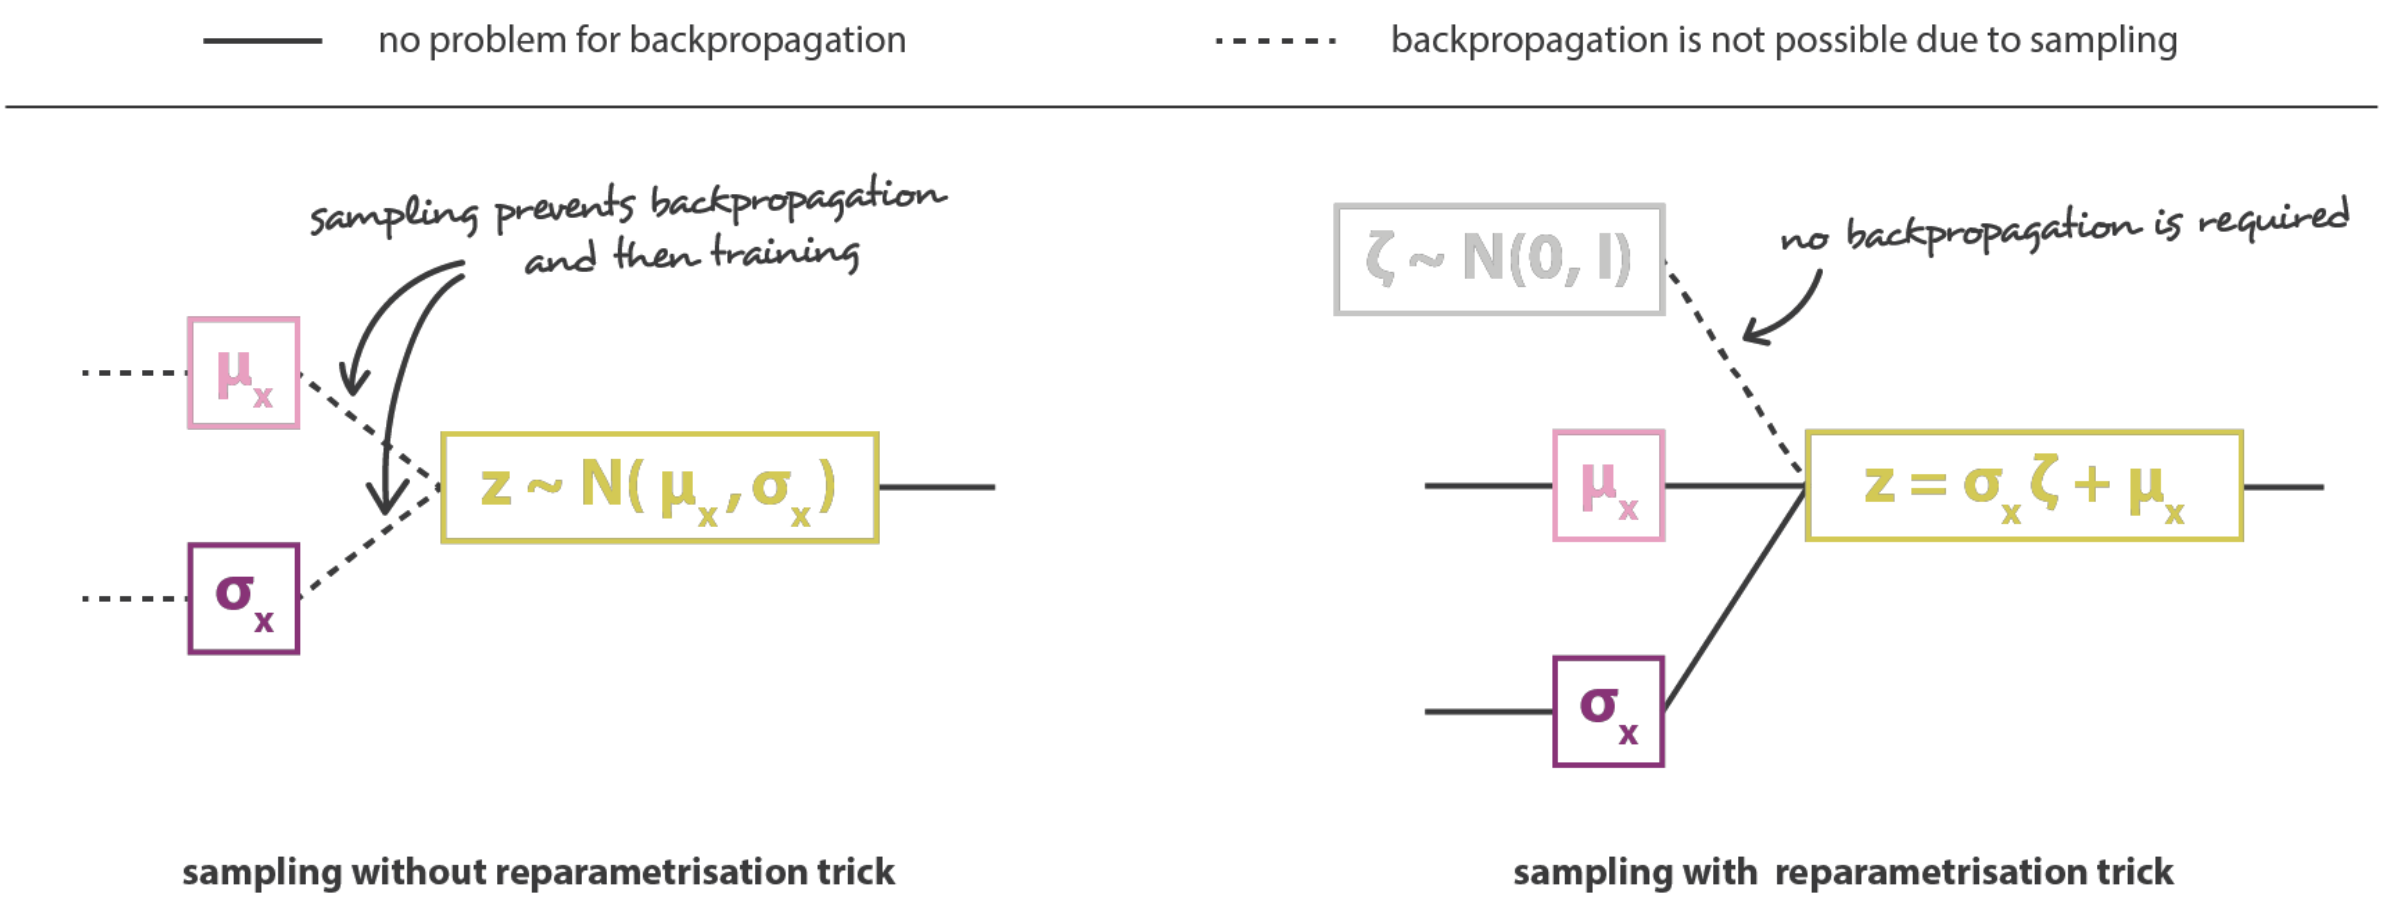
\includegraphics[width=\textwidth]{figure/RepTrick.png}
\caption{Effetto del reparametrization trick nel rendere il campionamento differenziabile}
\label{fig:repTrick}
\end{figure}
